\documentclass{standalone}
\usepackage{graphicx}	
\usepackage{amssymb, amsmath, amsthm}
\usepackage{color}

\usepackage{tikz}
\usetikzlibrary{intersections, backgrounds}

\definecolor{light}{RGB}{220, 188, 188}
\definecolor{mid}{RGB}{185, 124, 124}
\definecolor{dark}{RGB}{143, 39, 39}
\definecolor{gray60}{gray}{0.6}
\definecolor{gray70}{gray}{0.7}
\definecolor{gray80}{gray}{0.8}
\definecolor{gray90}{gray}{0.90}
\definecolor{gray95}{gray}{0.95}

\newcommand{\mcpoint}[2]{  
  \fill[color=dark] (#1, #2) circle (7pt); 
  \fill[color=light] (#1, #2) circle (5pt);
}

\begin{document}

\begin{tikzpicture}[scale=0.25, thick]
  %\draw[blue] (-12, -9.5) rectangle (12, 6.5);
  
  \foreach \i in {1, 0.99, ..., 0} {
    \pgfmathsetmacro{\prop}{100 * exp(-10.0 * \i * \i)};
    \colorlet{custom}{dark!\prop!white};
    \begin{scope}
      \clip (-0.005, -9.5) rectangle (12, 6.5);
      \draw[line width={30 * \i}, color=custom] 
      (0, 5) .. controls (5, 5) and (10, 8) .. (10, 0)
               .. controls (10, -8) and (5, -3) .. (-2, -10);
    \end{scope}
  
    \begin{scope}
      \clip (0.005, -9.5) rectangle (-12, 6.5);
      \draw[line width={30 * \i}, color=custom] 
      (0, 5) .. controls (-5, 5) and (-10, 8) .. (-10, 0)
               .. controls (-10, -8) and (-5, -3) .. (2, -10);
    \end{scope}
  }  
  \fill[opacity=0.3, green] (0, -8.5) circle (1);
  
  \draw[<-, >=stealth, line width=0.5] (-11, -5) -- (-11, -8.5)
  node[right] {$\varpi_{v}(q)$};
  
  \mcpoint{-8}{5.5}
  \mcpoint{-9}{4.75}
  \mcpoint{-8.7}{4.6}
  \mcpoint{-9.1}{4.5}
  \mcpoint{-9.2}{3.5}
  \mcpoint{-9.9}{3}
  \mcpoint{-9.6}{1.5}
  \mcpoint{-9.6}{1.5}
  \mcpoint{-9.75}{1}
  \mcpoint{-10.2}{0.25}
  \mcpoint{-9.8}{0}
  \mcpoint{-10}{-0.5}
  \mcpoint{-9.75}{-2}
  \mcpoint{-9.9}{-3}
  \mcpoint{-9.25}{-3.5}
  \mcpoint{-9}{-4.25}  
  \mcpoint{-8}{-4.5}
  \mcpoint{-8.25}{-4.75}
  \mcpoint{-7.75}{-5}
  \mcpoint{-6.5}{-5.5}
  \mcpoint{-5.75}{-5.25}
  \mcpoint{-5}{-6}
  \mcpoint{-4.75}{-6.25}
  \mcpoint{-3.8}{-6}
  \mcpoint{-3.25}{-6.5}
  \mcpoint{-2.75}{-6.75}
  \mcpoint{-2}{-7.5}
  \mcpoint{-1.75}{-6.8}
  \mcpoint{-1.5}{-7.2}
  
  %\draw[blue] (16, -9.5) rectangle (40, 6.5);

  \node[] at (30,-2) {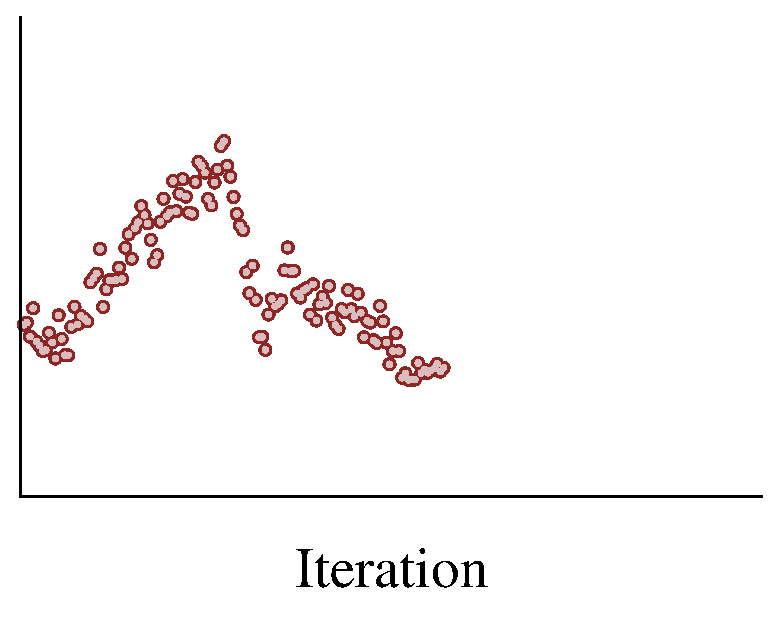
\includegraphics[width=5cm]{gnuplot/funnel_trace1.eps}};
  \node[rotate=90] at (18.5, -1) { $\varpi_{v}(q)$ };
  
  %\draw[blue] (44, -9.5) rectangle (68, 6.5);
  
  \node[] at (57,-2) {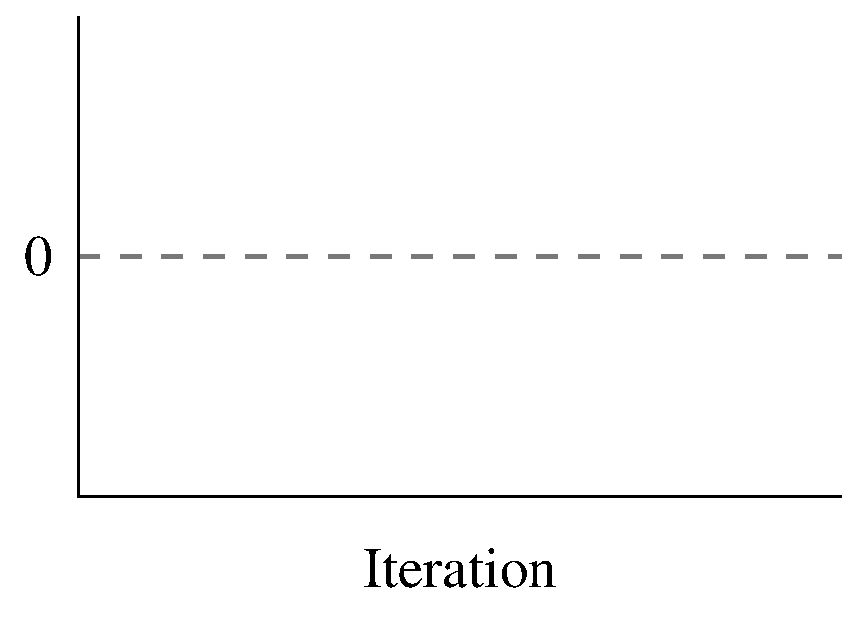
\includegraphics[width=5.5cm]{gnuplot/funnel_bias_axes.eps}};
  \node[rotate=90] at (44.5, -0.75) { $\mathbb{E} \! \left[ \varpi_{v} \right] - \hat{\varpi}_{v}$ };
  
  \draw[-,color=black, line width=0.5] (47.625, 4)
                                       .. controls (49, 1.5) and (56, 1.5) 
                                       .. (59.3, 1.5);
\end{tikzpicture}

\end{document}  